%% Grady Wright
%% Boise State University

%% Solutions by Sage Shaw
%% Boise State University

\documentclass[final,oneside,onecolumn]{article}
\usepackage[body={6in,9.5in},top=0.9in,left=1in,dvips]{geometry}
\usepackage{amsmath}
\usepackage{float}
\usepackage{graphicx}
\usepackage{amsfonts}
\usepackage{amssymb}
\usepackage{paralist}
\usepackage{floatflt}
\usepackage{alltt}
\usepackage{color}
%\usepackage{algorithm}
%\usepackage{algorithmic}
\usepackage{url}
\usepackage{xspace}
\definecolor{string}{rgb}{0.7,0.0,0.0}
\definecolor{comment}{rgb}{0.13,0.54,0.13}
\definecolor{keyword}{rgb}{0.0,0.0,1.0}

% Python LstListing
\definecolor{pygreen}{rgb}{0,.4,0}
\definecolor{pyoperator}{rgb}{.8,0,.8}
\definecolor{pycomment}{rgb}{.5,.5,.5}
\definecolor{pyidentifier}{rgb}{0,0,1}
\usepackage{listings}
\usepackage{courier}
\lstset{language=Python,
    keywordstyle=\color{pygreen},
    stringstyle=\color{string},
    commentstyle=\color{pycomment},
    %identifierstyle=\color{pyidentifier},
    literate=    {+}{{{\color{pyoperator}+}}}{1}
    {*}{{{\color{pyoperator}*}}}{1}
    {-}{{{\color{pyoperator}-}}}{1}
    {/}{{{\color{pyoperator}/}}}{1}
    {**}{{{\color{pyoperator}**}}}{2}
    {@}{{{\color{pyoperator}@}}}{1},
    basicstyle=\footnotesize\ttfamily\bfseries
}


\newcommand{\matlab}{{\sc Matlab}\xspace}
\newcommand{\matlabs}{\textsc{Matlab}'s\xspace}
\newcommand{\grads}{[\text{565 only}]}
\newcommand{\ugrads}{[\text{465 only}]}
\newcommand{\maple}{\emph{Maple\;}}
\newcommand{\erf}{\text{erf}}
\newcommand{\sign}{\text{sign}}
\newcommand{\lnorm}{\left\|}
\newcommand{\rnorm}{\right\|}
\newcommand{\ds}{\displaystyle}
\newcommand{\lam}{\lambda}
\newcommand{\ol}{\overline}
\newcommand{\vf}{\mathbf{f}}
\newcommand{\vy}{\mathbf{y}}
\newcommand{\vx}{\mathbf{x}}
\newcommand{\vd}{\mathbf{d}}
\newcommand{\sn}{\text{sn}}
\newcommand{\cn}{\text{cn}}
\newcommand{\dn}{\text{dn}}

\newcommand{\fdst}[3]{\left[\begin{array}{ccc} #1 & #2 & #3 \end{array}\right]}

\begin{document}

\renewcommand{\arraystretch}{0.5}

\title{\begin{tabular*}{6.5in}[h]{l@{\extracolsep\fill}cr}
{\bf \large Math 567} & {\bf \large Homework 6} & {\bf \large Due Nov.\ 30, 2018} \\
{\bf \large Problems by Grady Wright} \\
{\bf \large Solutions by Sage Shaw} \\
\end{tabular*}}
\date{}
\author{}
\maketitle

\thispagestyle{empty}

\medskip

\begin{enumerate}
%%%%%%%%%%%%%%%%%%%%%%%%%%%%%%%%%%%%%%%%%%%%%%%%%%%%%%%%%%%%%%%%%%%%%%%%%%%%%%%%%%%%%%%%%%%%%%%%%%%%%%%
\item \textbf{Crank-Nicolson}
\begin{enumerate}

\item Implement a function for numerically solving the solving the 1-D heat equation
\begin{equation*}
\begin{array}{lll}
u_t = \alpha u_{xx}, & a \leq x \leq b,\;\;\; t \geq 0, \\
u(x,0) = f(x), & u(a,t)=g_0(t),\; u(b,t)=g_1(t)\;. &
\end{array}
\end{equation*}
using  the Crank-Nicolson scheme (i.e. second order finite difference for the spatial derivative and trapezoidal rule for the time derivative). Your function should take as input: functions representing the initial
condition and boundary conditions, the number of points for the uniform spatial
discretization ($m+1$), the time span to solve the problem over, and the number of time
steps ($N$).  It should return the approximate solution at each time step (a matrix),
a vector containing all the time steps, and a vector containing the spatial
discretization. If using \matlab, then a possible function declaration is
\begin{quote}
\verb|[u,t,x] = cnhteq(f,g0,g1,tspan,alp,N,m)|
\end{quote}
The function should use a sparse matrix library or the fast discrete sine transform (DST) to solve the linear system that results from the implicit discretization.  Hand-in a copy of your
function and e-mail it to me.
{\small 
\begin{quote}
If possible, reuse your code from homework 3 for the differentiation
matrix of $u_{xx}$.
\end{quote}}

\bigbreak
\textit{Solution}:
\begin{lstlisting}[language=Python]
def cnhteq(initial, a, b, boundary_a, boundary_b, 
    coeff=1, target_time=1, N=10, m=16):
    
    ts = np.linspace(0, target_time, N+1)
    xs = np.linspace(a, b, m+2)
    
    h = (b-a)/(m+1)
    k = target_time/N
    
    us = np.zeros((N+1,m+2))
    us[:,0] = boundary_a(ts)
    us[:,-1] = boundary_b(ts)
    us[0, 1:-1] = initial(xs[1:-1])
    
    A = .5*coeff*k/h**2 * sp.diags([ [-2]*m, [1]*(m-1), [1]*(m-1) ], 
            offsets=[0,1,-1], format='csr')

    for i in range(1, N+1):
        rhs = (sp.eye(m) + A) @ us[i-1, 1:-1]
        rhs[0]  += coeff*k/h**2 * (us[i-1, 0] + us[i, 0])/2
        rhs[-1] += coeff*k/h**2 * (us[i-1, -1] + us[i, -1])/2
        us[i, 1:-1] = spla.spsolve(sp.eye(m) - A, rhs)
    return us, xs, ts
\end{lstlisting}



\bigbreak
%%%%%%%%%%%%%%%%%%%%%
\item Test your function on 1-D heat equation
\begin{equation*}
\begin{array}{lll}
u_t = u_{xx}, & 0 \leq x \leq 1,\;\;\; t \geq 0, \\
u(x,0) = \sin \frac{\pi x}{2} + \frac{1}{2}\sin 2\pi x, & u(0,t)=0,\; u(1,t)=e^{-\pi^2 t/4}\;,
\end{array}
\end{equation*}
which has the exact solution
\begin{equation*}
u(x,t) = e^{-\pi^2 t/4} \sin \frac{\pi x}{2} + \frac{1}{2} e^{-4\pi^2 t} \sin 2\pi x.
\end{equation*}
Use a \verb|waterfall| plot to plot the Crank-Nicolson solution
of the problem over the interval $0 \leq t \leq 1$ for $k=1/16$ and $h=1/16$.
Illustrate the second order accuracy of the method by computing the relative errors in the solution at $t=1$ for $h=k=2^{-n}$, $n=4,5,6,7,8$.  Produce a table or plot clearly showing the second order accuracy.
\end{enumerate}
\bigbreak

\textit{Solution}: Below can be seen the requested waterfall plot.
\begin{figure}[H]
    \centering
    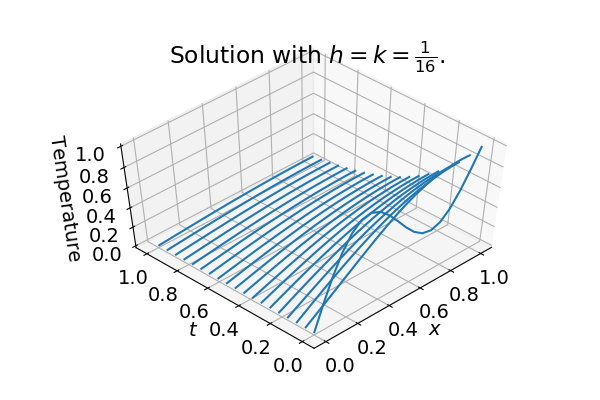
\includegraphics[width=.8\linewidth]{hw6_p1b_waterfall}
    %\captionof{figure}{A figure}
\end{figure}
The initial temperature distribution diffuses very rapidly and after the first curve in the plot no longer resembles the shape of the initial distribution. To better see the diffusion, I've included an animation in the file \texttt{hw6\_p1.mp4} that shows the diffusion using $N=1000$ and $m=100$. In the animation the diffusion is much more clearly seen.
\bigbreak

The second order convergence is clearly seen in the plot below in which the error in the method is plotted using values of $h=k = 2^{-n}$ with $n= 4,5,..., 9$. One extra data point was included to better estimate the order of convergence.
\begin{figure}[H]
    \centering
    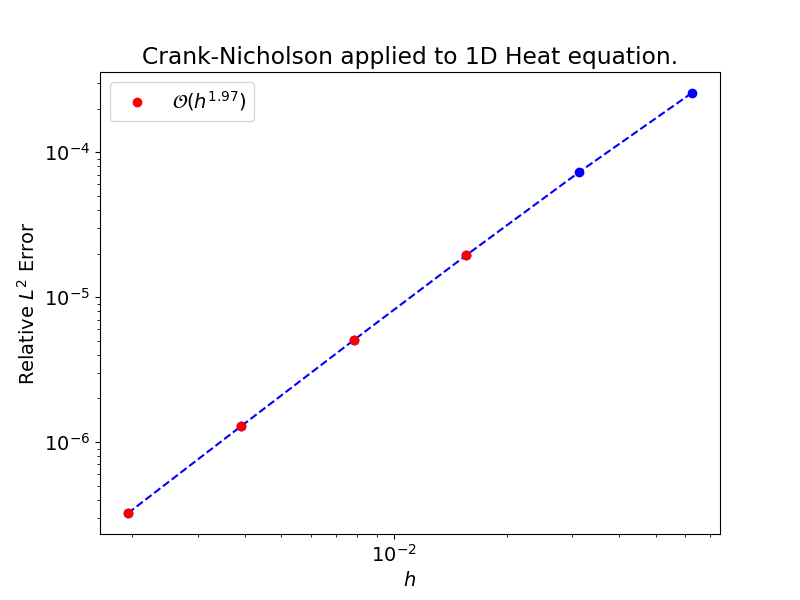
\includegraphics[width=.8\linewidth]{hw6_p1b_convergence}
    %\captionof{figure}{A figure}
\end{figure}

\medskip

%%%%%%%%%%%%%%%%%%%%%%%%%%%%%%%%%%%%%%%%%%%%%%%%%%%%%%%%%%%%%%%%%%%%%%%%%%%%%%%%%%%%%%%%%%%%%%%%%%%%%%%
\item Repeat problem 1, but use BDF2 for the time-integrator instead of trapezoidal rule.  To bootstrap this method use one initial step with Crank-Nicolson.  You do not need to produce a \verb|waterfall| plot, but you do need to illustrate the second order accuracy.  Which method is more accurate?
\bigbreak

\textit{Solution}:
\begin{lstlisting}[language=Python]
def bdf2_hteq(initial, a, b, boundary_a, boundary_b, 
    coeff=1, target_time=1, N=10, m=16):
    
    ts = np.linspace(0, target_time, N+1)
    xs = np.linspace(a, b, m+2, endpoint=True)
    
    h = (b-a)/(m+1)
    k = target_time/N
    
    us = np.zeros((N+1,m+2))
    us[:,0] = boundary_a(ts)
    us[:,-1] = boundary_b(ts)
    us[0, 1:-1] = initial(xs[1:-1])
    
    # one step of cn
    A = coeff*k/h**2 * sp.diags([ [-2]*m, [1]*(m-1), [1]*(m-1) ], 
offsets=[0,1,-1], format='csr')
    for i in range(1, 2):
        rhs = (sp.eye(m) + .5*A) @ us[i-1, 1:-1]
        rhs[0]  += coeff*k/h**2 * (us[i-1, 0] + us[i, 0])/2
        rhs[-1] += coeff*k/h**2 * (us[i-1, -1] + us[i, -1])/2
        us[i, 1:-1] = spla.spsolve(sp.eye(m) - .5*A, rhs)
    
    # BDF2
    for i in range(2, N+1):
        rhs = (4*us[i-1, 1:-1] - us[i-2, 1:-1])/3
        rhs[0]  += 2/3 * coeff*k/h**2 * us[i, 0]
        rhs[-1] += 2/3 * coeff*k/h**2 * us[i, -1]
        us[i, 1:-1] = spla.spsolve(sp.eye(m) - 2/3*A, rhs)
    
    return us, xs, ts
\end{lstlisting}
Below is the plot verifying second order accuracy. Thought they are both second order, Crank-Nicholson appears to be better by roughly an order of magnitude.
\begin{figure}[H]
    \centering
    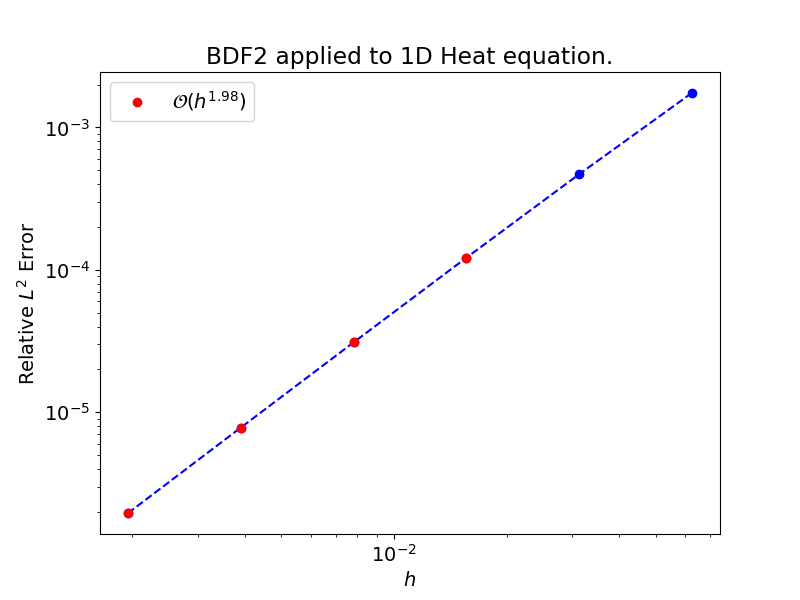
\includegraphics[width=.8\linewidth]{hw6_p2_convergence}
    %\captionof{figure}{A figure}
\end{figure}

%%%%%%%%%%%%%%%%%%%%%%%%%%%%%%%%%%%%%%%%%%%%%%%%%%%%%%%%%%%%%%%%%%%%%%%%%%%%%%%%%%%%%%%%%%%%%%%%%%%%%%%
\item \textbf{Linear stability analysis} To numerically solve
the equation
\begin{equation*}
\begin{array}{lll}
u_t + u_{xxx} = 0, & 0 \leq x \leq 1, & t \geq 0, \\
u(x,0) = g(x), & u(0,t) = u(1,t) &
\end{array}
\end{equation*}
with periodic boundary conditions, a \emph{naive} numerical analyst proposes to use
the simple scheme of forward Euler in time and centered, second-order differences
in space:
\begin{equation*}
\dfrac{u(x,t+k) - u(x,t)}{k} + \dfrac{-\frac{1}{2}u(x-2h,t) + u(x-h,t) - u(x+h,t) + \frac{1}{2}u(x+2h,t)}{h^3} = 0\;.
\end{equation*}
\begin{enumerate}
\item Using some general principles about numerical stability of IVP solvers, explain to the numerical analyst that
this scheme is unconditionally unstable, and thus should never be used.

\bigbreak
\textit{Solution}: The second order approximation to $u_{xxx}$ leads to a skew-symmetric differentiation matrix. The eigenvalues of a such a matrix will be purely imaginary and thus this method will never satisfy the stability criterion for Forward Euler. In fact, any order of finite difference approximation to $u_{xxx}$ on an equispaced grid will be skew-symmetric and thus Forward Euler will fail for all of them.

\bigbreak
%%%%%%%%%%%%%%%%%%%%%
\item Propose an alternative scheme that can be used to successfully approximate this PDE (i.e.\ give a scheme that is conditionally or unconditionally stable).
\bigbreak

\textit{Solution}: Backward Euler will be unconditionally stable for the same reason since the entire imaginary axis is in the stability domain of Backward Euler. Leap-Frog would be conditionally stable since it's stability domain is the imaginary axis between $i$ and $-i$.

\end{enumerate}

\medskip

%\item As discussed in class, the upwind scheme for the advection 
%equation 
%\begin{equation*}
%u_t + c u_x = 0\;\;(c > 0)
%\end{equation*}
%is only first order accurate in space and time (and highly diffusive).  The 
%so called box scheme is similar to the upwind scheme, except that 
%it is second order accurate in space and time.  The main difference, however, is 
%that it is implicit.  If $c>0$ then the scheme is given as 
%\begin{multline}
%\frac{1}{2}\left(\frac{u(x,t+k)-u(x,t)}{k} + \frac{u(x-h,t+k)-u(x-h,t)}{k}\right) = \\
%\frac{c}{2}\left(\frac{u(x-h,t+k)-u(x,t+k)}{h} + \frac{u(x-h,t)-u(x,t)}{h}\right).
%\label{box_scheme}
%\end{multline}
%One can view this as averaging the backward (upwinded) spatial derivative at time $t+k$
%and $t$ and averaging the time derivative at $x-h$ and $x$.  Note that if $c<0$,
%one would instead use averaging of the forward (downwinded) spatial derivative and
%time averaging about $x$ and $x+h$.
%\begin{enumerate}
%\item Using Maple or Mathematica, show that the box scheme is second order accurate in space 
%and time.  The easiest way to perform this task is to do a two-dimensional 
%Taylor series expansion of (\ref{box_scheme}) in $h$ and $k$ using the Maple function
%\texttt{mtaylor} or the Mathematica function \texttt{Series}.  Then use the advection equation to eliminate any $O(h)$ or $O(k)$
%terms.
%
%\item Draw the stencil for the Box scheme and then determine its stability restriction
% imposed by the CFL condition.
%
%\item Using von Neumann stability analysis, determine the correct stability 
%restriction on the Box scheme.
%\end{enumerate}


%%%%%%%%%%%%%%%%%%%%%%%%%%%%%%%%%%%%%%%%%%%%%%%%%%%%%%%%%%%%%%%%%%%%%%%%%%%%%%%%%%%%%%%%%%%%%%%%%%%%%%%
 \item \textbf{Wave equation, part I} Initial value problems (IVPs) of the form 
 \begin{align*}
 y'' = f(t,y,y'),\; t \geq t_0,\; y(t_0)=y_0,\; y'(t_0) = y_0'
 \end{align*}
 can be solved directly without converting to a first order system using a generalization of Runge-Kutta methods known as Nystr\"om methods. In contrast to explicit RK methods for $y'=f(t,y)$, these can be of higher order than  their number of stages.  When the RHS of the IVP does not depend on $y'$ (i.e.\ $y'' = f(t,y)$), explicit Runge-Kutta-Nystr\"om (RKN) methods can be particularly effective. One well-known RKN method for these types of problems is defined by the Butcher diagram
 \begin{equation*}
 \renewcommand{\arraystretch}{1.1}
 \begin{array}{c|ccc}
 0 & \\
 \frac{1}{2} & \frac{1}{8} \\
 1 & 0 & \frac{1}{2} \\
 \hline
   & \frac{1}{6} & \frac{1}{3} & 0 \\
 \hline
   & \frac{1}{6} & \frac{2}{3} & \frac{1}{6}
 \end{array}
 \end{equation*}
 This translates into the scheme:
 \begin{align*}
 d_1 &= f(t_n, y^{n})  \\
 d_2 &= f\left(t_n+\frac{k}{2}, y^{n}+\frac{k}{2} (y')^n + \frac{k^2}{8}d_1\right) \\
 d_3 &= f\left(t_n+k, y^{n}+k (y')^n +\frac{k^2}{2}d_2\right) \\
 y^{n+1} &= y^{n} + k (y')^n + k^2\left(\frac{1}{6}d_1 + \frac{1}{3}d_2\right) \\
 (y')^{n+1} &= (y')^{n} + k\left(\frac{1}{6}d_1 + \frac{2}{3}d_2 + \frac{1}{6} d_3 \right)
 \end{align*}
 One can show that this scheme is fourth-order accurate even though it has only three stages.
 
 \begin{enumerate}
\item Write a function that combines RKN scheme above with fourth-order accurate finite differences in space to numerically solve the second-order wave equation
 \begin{align}
 u_{tt} = c^2 u_{xx},\; 0 \leq x < 2\pi,\; t> 0,\; u(x,0) = f(x),\; u_t(x,0) = g(x)
 \label{eq:wave_eq}
 \end{align}
with \emph{periodic} boundary conditions.  For reference, the fourth-order accurate centered finite difference formula is
\begin{align*}
u''(x) = \frac{1}{12h^2}\left[-u(x-2h) + 16 u(x-h) - 30 u(x) + 16 u(x+h) - u(x+2h)\right] + \mathcal{O}(h^4).
\end{align*}
Solve the problem on the equispaced grid $x_j = jh$, $j=0,\ldots,m$, where $h=2\pi/(m+1)$.
\bigbreak

\textit{Solution}:
\begin{lstlisting}[language=Python]
def RKN_wave(init_dis, init_vel, coeff=1, target_time=2*np.pi, N=10, m=16):
    ts = np.linspace(0, target_time, N+1)
    xs = np.linspace(0, 2*np.pi, m+1, endpoint=False)
    
    h = (2*np.pi)/(m+1)
    k = target_time/N
    
    us = np.zeros((N+1,m+1))
    us[0] = init_dis(xs)
    u_prime = init_vel(xs)
    
    A = sp.diags(
        [ [-30]*(m+1), [16]*(m-0), [16]*(m-0), [-1]*(m-1), [-1]*(m-1) ], 
        offsets=[0,1,-1, 2, -2], format='lil')
    A[ 0, -1] = 16
    A[ 0, -2] = -1
    A[ 1, -1] = -1
    A[-2,  0] = -1
    A[-1,  0] = 16
    A[-1,  1] = -1
    A *= coeff**2 / (12*h**2)
    A = A.tocsr()
    
    for i in range(1, N+1):
        d1 = A @ us[i-1]
        d2 = A @ (us[i-1] + k/2*u_prime + k**2/8*d1)
        d3 = A @ (us[i-1] + k*u_prime + k**2/2*d2)
        us[i] = us[i-1] + k*u_prime + k**2*(1/6*d1 + 1/3*d2)
        u_prime = u_prime + k*(1/6*d1 + 2/3*d2 + 1/6*d3)
    
    return us, xs, ts
\end{lstlisting}

\bigbreak
%%%%%%%%%%%%%%%%%%%%%
\item \label{prob:wave_eq} Use your function to solve the wave equation with $m=200$, wave speed $c=1$, and the initial conditions\footnote{The initial condition $f(x)$ is not technically periodic, but it looks periodic to machine precision.}
\begin{align*}
f(x) = \exp(-20(x-\pi/2)^2) + \frac32 \exp(-20(x-4\pi/3)^2),\; g(x) = 0.
\end{align*}
Solve the problem for $0 \leq t \leq 2\pi$ using a time-step of $k=2\pi/400$.  Produce a \verb|waterfall| plot of the solution.  Also plot the error in the solution at $t=2\pi$.  You can do this by simply computing the difference between the numerical solution at $t=2\pi$ and the initial condition.
\bigbreak

\textit{Solution}: The waterfall plot below shows the solution to the given specifications.
\begin{figure}[H]
    \centering
    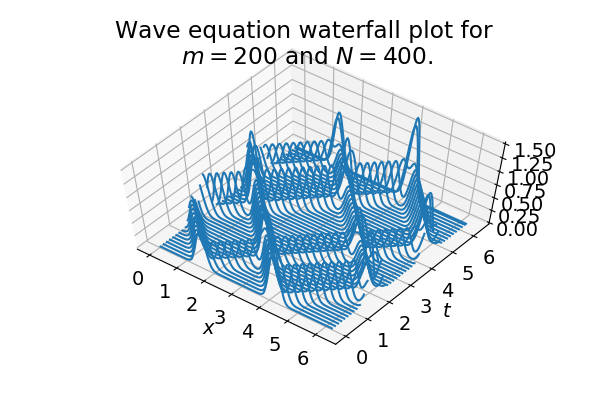
\includegraphics[width=.8\linewidth]{hw6_p4b_waterfall}
\end{figure}
As before, I feel like waterfall plots are inferior to animations in illustrating a solution. I've included a very satisfying animation of the solution in the file \texttt{hw6\_p4.mp4}.\\
Below is the error plot at the final timestep.
\begin{figure}[H]
    \centering
    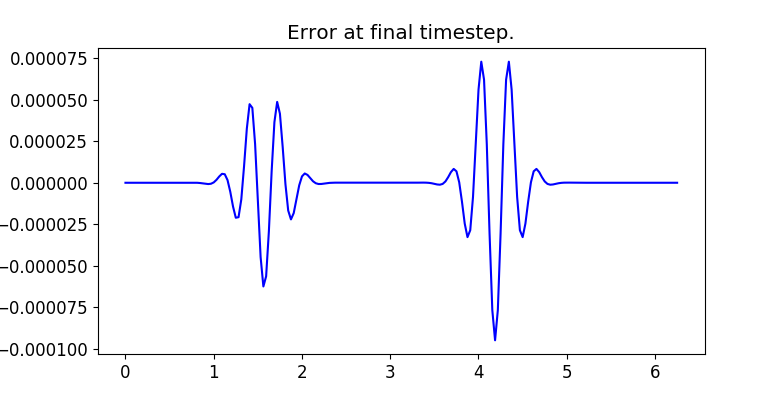
\includegraphics[width=.8\linewidth]{hw6_p4b_error}
\end{figure}

\bigbreak
%%%%%%%%%%%%%%%%%%%%%
\item \label{prob:wave_eq_fourier}  Extra credit:  Since the domain is periodic, we can greatly increase the accuracy of the spatial derivative approximation without much worry about stability.  For this extra credit problem, replace the fourth-order finite difference approximation with a Fourier spectral method approximation of $u''(x)$ and repeat part (b).
\end{enumerate}
\bigbreak

\textit{Solution}:
\begin{lstlisting}[language=Python]
def RKN_wave_FFT(init_dis, init_vel, coeff=1, target_time=2*np.pi, N=10, m=16):
    ts = np.linspace(0, target_time, N+1)
    xs = np.linspace(0, 2*np.pi, m+1, endpoint=False)
    
    h = (2*np.pi)/(m+1)
    k = target_time/N
    
    us = np.zeros((N+1,m+1))
    us[0] = init_dis(xs)
    u_prime = init_vel(xs)
    
    for i in range(1, N+1):
        d1 = coeff**2 * fft.diff(us[i-1], order=2)
        d2 = coeff**2 * fft.diff(us[i-1] + k/2*u_prime + k**2/8*d1, order=2)
        d3 = coeff**2 * fft.diff(us[i-1] + k*u_prime + k**2/2*d2, order=2)
        us[i] = us[i-1] + k*u_prime + k**2*(1/6*d1 + 1/3*d2)
        u_prime = u_prime + k*(1/6*d1 + 2/3*d2 + 1/6*d3)
    
    return us, xs, ts
\end{lstlisting}
The plots below show the solution using the Fourier spectral approximation to $u''(x)$ and the error in the final timestep.
\begin{figure}[H]
	\centering
	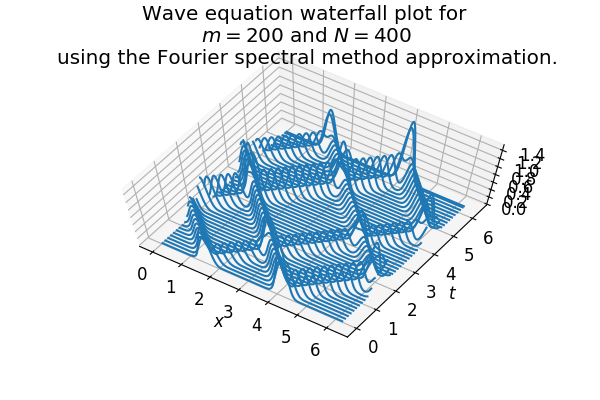
\includegraphics[width=.8\linewidth]{hw6_p4c_waterfall}
\end{figure}
\begin{figure}[H]
	\centering
	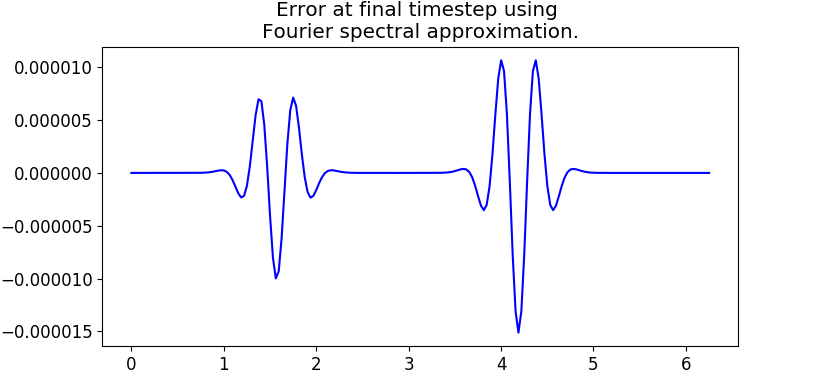
\includegraphics[width=.8\linewidth]{hw6_p4c_error}
\end{figure}

%%%%%%%%%%%%%%%%%%%%%%%%%%%%%%%%%%%%%%%%%%%%%%%%%%%%%%%%%%%%%%%%%%%%%%%%%%%%%%%%%%%%%%%%%%%%%%%%%%%%%%%
\item \textbf{Wave equation, part II}

\begin{enumerate}
\item Show that the wave equation \eqref{eq:wave_eq} can be transformed into the equivalent first order system of two equations, given by
\begin{equation}
\begin{aligned}
u_t + v_x & = & 0 \\
v_t + c^2 u_x & = & 0
\end{aligned}
\label{eqn:oneway}
\end{equation}
\noindent
subject to $u(x,0) = f(x)$, $v(x,0) = G(x) = -\int g(x) dx$ for functions $u(x,t)$ and $v(x,t)$.  This is a linear, constant coefficient
hyperbolic system of the form
\begin{equation}
q_t + Aq_x = 0
\label{eqn:sys}
\end{equation}
\noindent
where $A$ is a $2 \times 2$ matrix and $q(x,t) = (u(x,t),v(x,t))$.
\bigbreak

\textit{Solution}: We begin with the differential equation
$$
u_{tt} = c^2u_{xx}
$$
with the initial conditions of $u(x,0) = f(x)$ and $u_t(x,0) = g(x)$ subject to periodic boundary conditions.\\
Let $v(x,t) = -\int u_t(x,t) dx$. Choose the constant arbitrarily as it will not affect the solution of $u$, only the solution of $v$. It then follows that $v_x = -u_t$ or equivalently $u_t + v_x = 0$. \\
Also it is the case that $v_t = -\int u_tt dx$. If we anti-differentiate both sides of our differential equation we have
\begin{align*}
	u_{tt} &= c^2u_{xx} \\
	\int u_{tt} dx &= c^2 u_x \\
	-v_t &= c^2 u_x \\
	0 &= v_t + c^2 u_x
\end{align*}
Thus we have derived the system of differential equations as desired. The initial condition is similarly shown: $G(x) = v(x,0) = -\int u_t(x,0) dx = -\int g(x) dx$.


\bigbreak
%%%%%%%%%%%%%%%%%%%%%
\item Write a function for numerically solving \eqref{eqn:oneway} using fourth-order centered finite differences in space and the standard fourth order Runge-Kutta (RK4) method in time.  
For reference, the fourth-order accurate centered finite difference formula is
\begin{align*}
u'(x) = \frac{1}{12h}\left[u(x-2h) -  8u(x-h)  + 8 u(x+h) - u(x+2h)\right] + \mathcal{O}(h^4).
\end{align*}
As in the previous problem, compute the solution on the equispaced grid $x_j = jh$, $j=0,\ldots,m$, where $h=2\pi/(m+1)$.
\bigbreak

\textit{Solution}:
\begin{lstlisting}[language=Python]
def RKN_wave_sys(init_dis, int_init_vel, coeff=1, target_time=2*np.pi, N=10, m=16):
	ts = np.linspace(0, target_time, N+1)
	xs = np.linspace(0, 2*np.pi, m+1, endpoint=False)
	
	h = (2*np.pi)/(m+1)
	k = target_time/N
	
	# qs contain us in the first m+1 cols and vs in the rest
	qs = np.zeros( (N+1,(m+1)*2) )
	qs[0,:m+1] = init_dis(xs)
	qs[0,m+1:] = int_init_vel(xs)
	
	A = sp.diags(
		[ [1]*(m-1), [-8]*(m-0), [8]*(m-0), [-1]*(m-1) ], 
		offsets=[-2, -1, 1, 2], format='lil')
	A[ 0, -1] = -8
	A[ 0, -2] =  1
	A[ 1, -1] =  1
	A[-2,  0] = -1
	A[-1,  0] =  8
	A[-1,  1] = -1
	A *= -1 / (12*h)
	A = sp.bmat([[None, A],[coeff**2*A, None]]).tocsr()
	
	for i in range(1,N+1):
		k1 = k * A@ qs[i-1]
		k2 = k * A@(qs[i-1] + k1/2)
		k3 = k * A@(qs[i-1] + k2/2)
		k4 = k * A@(qs[i-1] + k3)
		qs[i] = qs[i-1] + k1/6 + k2/3 + k3/3 + k4/6
	
	return qs[:,:m+1], xs, ts 
\end{lstlisting}

\bigbreak
%%%%%%%%%%%%%%%%%%%%%
\item Repeat \ref{prob:wave_eq}, but using your function from part (a) of this problem.
\bigbreak

\textit{Solution}:
Below can be seen the waterfall plot and the plot of the error after the final timestep.
\begin{figure}[H]
	\centering
	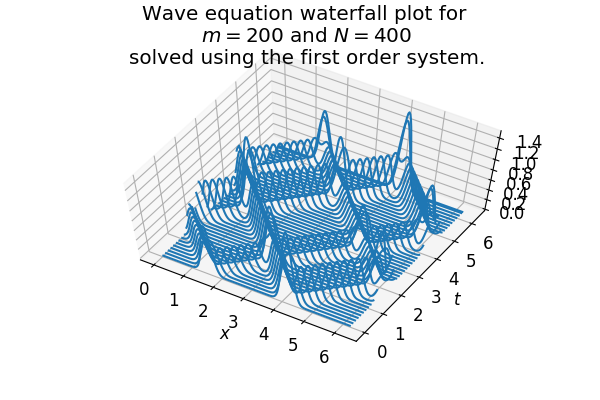
\includegraphics[width=.8\linewidth]{hw6_p5b_waterfall}
\end{figure}
\begin{figure}[H]
	\centering
	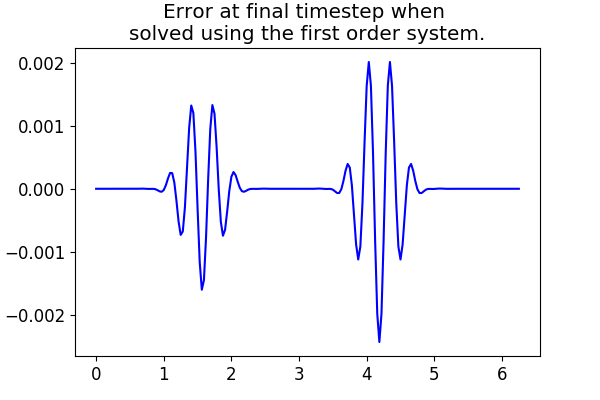
\includegraphics[width=.8\linewidth]{hw6_p5b_error}
\end{figure}

\bigbreak
%%%%%%%%%%%%%%%%%%%%%
\item While the two formulations \eqref{eqn:oneway} and \eqref{eq:wave_eq} are mathematically equivalent, numerical methods for solving them may not be.   Compare the solutions from part (c) and that of the previous problem to determine which method gives better accuracy.
\bigbreak

\textit{Solution}:
Solving the wave equation above using the system of first order equations give a relative error of 0.00145634, whereas solving it directly using the RKN scheme gives a relative error of 5.22702e-05 - much more accurate!

\bigbreak
%%%%%%%%%%%%%%%%%%%%%
\item Extra credit:  Similar to \ref{prob:wave_eq_fourier}, replace the fourth-order FD approximation of the spatial derivatives in \eqref{eqn:oneway} with a Fourier spectral method approximation.  Repeat part (c) with this approximation.
\bigbreak

\textit{Solution}:
\textit{Solution}:
\begin{lstlisting}[language=Python]
def RKN_wave_sys_FFT(init_dis, int_init_vel, coeff=1, target_time=2*np.pi, N=10, m=16):
	ts = np.linspace(0, target_time, N+1)
	xs = np.linspace(0, 2*np.pi, m+1, endpoint=False)
	
	h = (2*np.pi)/(m+1)
	k = target_time/N
	
	# qs contain us in the first m+1 cols and vs in the rest
	qs = np.zeros( (N+1,(m+1)*2) )
	qs[0,:m+1] = init_dis(xs)
	qs[0,m+1:] = int_init_vel(xs)
	
	A = sp.diags(
	[ [1]*(m-1), [-8]*(m-0), [8]*(m-0), [-1]*(m-1) ], 
	offsets=[-2, -1, 1, 2], format='lil')
	A[ 0, -1] = -8
	A[ 0, -2] =  1
	A[ 1, -1] =  1
	A[-2,  0] = -1
	A[-1,  0] =  8
	A[-1,  1] = -1
	A *= -1 / (12*h)
	A = sp.bmat([[None, A],[coeff**2*A, None]]).tocsr()
	
	k1 = np.zeros(qs[0].shape)
	k2 = np.zeros(qs[0].shape)
	k3 = np.zeros(qs[0].shape)
	k4 = np.zeros(qs[0].shape)
	
	for i in range(1,N+1):
		tmp = qs[i-1]
		k1[:m+1] = -k*           fft.diff(tmp[m+1:])
		k1[m+1:] = -k*coeff**2 * fft.diff(tmp[:m+1])
		tmp = qs[i-1] + k1/2
		k2[:m+1] = -k*           fft.diff(tmp[m+1:])
		k2[m+1:] = -k*coeff**2 * fft.diff(tmp[:m+1])
		tmp = qs[i-1] + k2/2
		k3[:m+1] = -k*           fft.diff(tmp[m+1:])
		k3[m+1:] = -k*coeff**2 * fft.diff(tmp[:m+1])
		tmp = qs[i-1] + k3
		k4[:m+1] = -k*           fft.diff(tmp[m+1:])
		k4[m+1:] = -k*coeff**2 * fft.diff(tmp[:m+1])
		qs[i] = qs[i-1] + k1/6 + k2/3 + k3/3 + k4/6
	
	return qs[:,:m+1], xs, ts 
\end{lstlisting}
Below can be seen the waterfall plot and the plot of the error after the final timestep.
\begin{figure}[H]
	\centering
	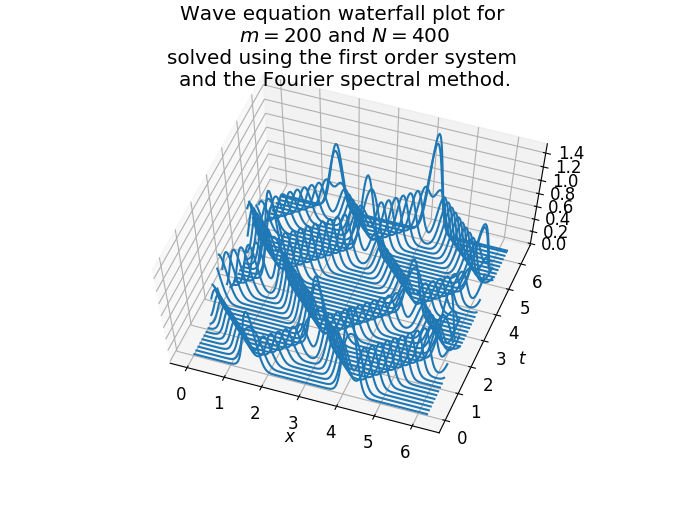
\includegraphics[width=.8\linewidth]{hw6_p5e_waterfall}
\end{figure}
\begin{figure}[H]
	\centering
	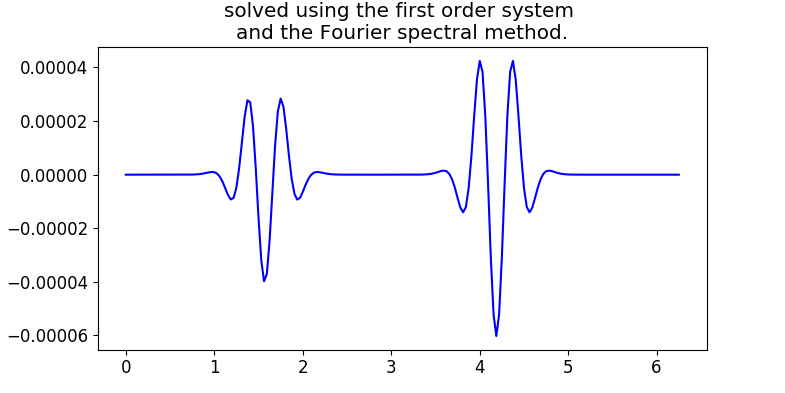
\includegraphics[width=.8\linewidth]{hw6_p5e_error}
\end{figure}
The final comparisons of all errors for solving the wave equation with $N=400$ and $m=200$ are given in the table below.

\begin{center}
	\begin{tabular}{|l|c|}
		\hline
		\textbf{Method} & \textbf{Relative Error}\\ \hline
		Fourth order (time and space) on \eqref{eq:wave_eq} & 5.22702e-05\\ \hline
		Fourth order (time and space) on \eqref{eqn:oneway} & 8.55204e-06\\ \hline
		Fourth in time, spectral in space on \eqref{eq:wave_eq} & 0.00145634\\ \hline
		Fourth in time, spectral in space on \eqref{eqn:oneway} & 3.40471e-05\\
		\hline
	\end{tabular}
\end{center}

Even using spectral accuracy in space the error when using the first order system of equations is worse than using the RKN scheme on the wave equation directly.


\end{enumerate}

\end{enumerate}

\end{document}
